\documentclass[../characterization.tex]{subfiles}
\graphicspath{{\subfix{../../../../images/}}}
\begin{document}
    \textbf{X-ray diffraction (XRD)}\cite{b11} is a widely used technique for characterizing the crystal structure, composition, and 
    phase identification of materials, including nanophosphors. It relies on the principle of X-ray scattering by 
    the crystal lattice, providing information about the spacing and arrangement of atoms within the material.
    X-ray diffraction is a powerful technique for investigating the crystallographic properties of nanophosphors, 
    including their crystal structure, phase composition, and crystallite size. It is a non-destructive and highly 
    informative characterization tool used in materials science, chemistry, geology, and many other fields. 
    Here is an overview of X-ray diffraction:
    \begin{Figure}
        \centering
        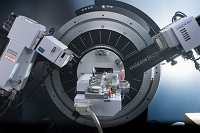
\includegraphics[width=0.6\linewidth]{xrd.jpg}
        \captionof{figure}{A X-ray diffraction machine\cite{u11}}\label{fig:xrd}
    \end{Figure}
    \begin{itemize}
        \item \textbf{Principle: } XRD involves exposing a sample to a beam of X-rays and measuring the resulting 
        diffraction pattern. X-rays interact with the crystal lattice, causing constructive interference of scattered 
        waves. The angles and intensities of the diffracted X-rays provide information about the crystal structure 
        and spacing of atomic planes.
        \item \textbf{Bragg's Law: }The diffraction pattern is described by Bragg's law, which relates the angle 
        of incidence ($\theta$), the wavelength of the X-rays ($\lambda$), and the distance between crystal planes 
        ($d$) in the material: $n{\lambda} = 2dsin(\theta)$, where n is an integer representing the order of 
        diffraction.
        \item \textbf{Sample Preparation: }he nanophosphor sample is typically prepared as a powder or thin film 
        to ensure a random orientation of the crystal planes. The sample should be finely ground to ensure a 
        homogeneous scattering of X-rays.
        \item \textbf{X-ray Source: }XRD uses a monochromatic X-ray source, often a high-intensity source like a 
        rotating anode X-ray tube or a synchrotron. The wavelength of the X-rays is selected depending on the 
        material and the desired diffraction information.
        \item \textbf{Diffraction Pattern Measurement: }The X-rays diffracted by the sample are captured by a 
        detector, typically a scintillation or solid-state detector. The detector records the intensity of the 
        diffracted X-rays as a function of the diffraction angle ($2\theta$). The diffraction pattern is a series 
        of peaks representing the diffracted intensity as a function of the diffraction angle.
        \item \textbf{Data Analysis: }The diffraction pattern is analyzed using specialized software to determine 
        the crystal structure and phase identification. The positions, intensities, and shapes of the diffraction 
        peaks are compared with reference databases to identify the crystal structure and phase composition of 
        the nanophosphor.
        \item \textbf{Quantitative Analysis: } XRD can also provide quantitative information about the crystalline 
        phases present in the sample. By comparing the intensity of the diffracted peaks with known standards or 
        through peak fitting analysis, the relative abundance of different phases can be determined.
    \end{itemize}
\end{document}